\documentclass[aspectratio=169, 11pt, t, xcolor={table}]{beamer}
% Slides of the English course "Computer Architecture" (same theme as the
% ENSB decks: light background, teal + orange). Compile from en/slides/.
\usepackage{amsmath, amssymb}
\usepackage{booktabs, colortbl, tabularx, array}
\usepackage{tikz}
\usepackage[skins]{tcolorbox}
\usepackage{fontawesome5}
\usepackage{listings}
\usepackage{fontspec}
\usetikzlibrary{positioning, calc, arrows.meta, shapes.geometric, decorations.pathreplacing}

\setsansfont{texgyreheros}[Extension=.otf, UprightFont=*-regular, BoldFont=*-bold,
    ItalicFont=*-italic, BoldItalicFont=*-bolditalic]
\newfontfamily\codefont[Scale=0.95, BoldFont=lmmonolt10-bold.otf,
    ItalicFont=lmmono10-italic.otf]{lmmono10-regular.otf}

\definecolor{brandTeal}{HTML}{5CC8E6}
\definecolor{brandOrange}{HTML}{FFA27F}
\definecolor{brandLight}{HTML}{F8F9FA}
\definecolor{brandDark}{HTML}{263238}
\definecolor{brandMuted}{HTML}{6C757D}
\definecolor{brandGreen}{HTML}{7BC47F}
\definecolor{brandPurple}{HTML}{B39DDB}
\colorlet{tealDeep}{brandTeal!60!black}
\colorlet{orangeDeep}{brandOrange!70!black}
\definecolor{codeGrey}{HTML}{F1F3F5}

\setbeamercolor{background canvas}{bg=brandLight}
\setbeamercolor{normal text}{fg=brandDark}
\setbeamercolor{structure}{fg=brandTeal}
\setbeamertemplate{navigation symbols}{}
\setbeamertemplate{frametitle}{%
    \vspace{0.35cm}
    \noindent{\bfseries\Large\color{brandDark}\insertframetitle}\par
    \vskip-2pt\noindent{\color{brandTeal}\rule{\textwidth}{1.5pt}}\vspace{0.05cm}}
\setbeamertemplate{footline}{%
    \hbox to \paperwidth{\hspace{0.6cm}{\color{brandMuted}\scriptsize\insertshorttitle}\hfill
        {\color{brandMuted}\scriptsize\insertframenumber\,/\,\inserttotalframenumber}\hspace{0.6cm}}%
    \vspace{0.25cm}}
\setbeamertemplate{itemize item}{\color{brandTeal}\small\faChevronRight}
\setbeamertemplate{itemize subitem}{\color{brandMuted}\small\faAngleRight}
\setbeamertemplate{enumerate item}{\color{tealDeep}\bfseries\insertenumlabel.}
% list lines are 1.4 cm apart (baseline to baseline)
\newlength{\lineGap}\setlength{\lineGap}{1.4cm}
\let\origlist\list
\def\list#1#2{\origlist{#1}{#2\setlength{\itemsep}{\dimexpr\lineGap-\baselineskip\relax}\setlength{\parsep}{0pt}}}

\newcolumntype{L}{>{\raggedright\arraybackslash}X}
\newcolumntype{C}{>{\centering\arraybackslash}X}
\newcommand{\ras}[1]{\cellcolor{brandTeal!20}\textbf{#1}}
\newcommand{\cell}[2]{\leavevmode\textcolor{#1}{#2}}
\renewcommand{\arraystretch}{1.3}
\setlength{\arrayrulewidth}{0.6pt}
\arrayrulecolor{brandMuted!70}

\tcbset{brandbox/.style={enhanced, arc=4pt, outer arc=4pt, boxrule=1.5pt,
    coltitle=white, coltext=brandDark, fonttitle=\bfseries,
    toptitle=0.8mm, bottomtitle=0.8mm, top=1.2mm, bottom=1.2mm, left=3mm, right=3mm,
    before skip=4pt, after skip=4pt}}
\newtcolorbox{tbox}[2][]{brandbox, colback=brandTeal!10, colframe=brandTeal, title={#2}, #1}
\newtcolorbox{obox}[2][]{brandbox, colback=brandOrange!10, colframe=brandOrange, title={#2}, #1}
\newtcolorbox{gbox}[2][]{brandbox, colback=brandGreen!8, colframe=brandGreen, title={#2}, #1}
\newtcolorbox{pbox}[2][]{brandbox, colback=brandPurple!10, colframe=brandPurple, title={#2}, #1}

\newcommand{\code}[1]{\mbox{\codefont\color{tealDeep}#1}}
\newcommand{\hex}[1]{\mbox{#1\textsubscript{H}}}
\newcommand{\bin}[1]{\mbox{#1\textsubscript{2}}}
\newcommand{\nql}[2]{\mbox{#1\,$\leftarrow$\,#2}}

% ---- code from ../../code/ (the verified programs of the course) ----
\lstdefinelanguage{asm86}{
    morekeywords={mov, add, adc, sub, sbb, inc, dec, neg, mul, imul, div, idiv,
        cmp, and, or, xor, not, test, shl, shr, sal, sar, rol, ror, jmp, je, jne,
        jz, jnz, jg, jge, jl, jle, ja, jae, jb, jbe, jcxz, loop, call, ret, iret,
        int, push, pop, lea, xchg, in, out, nop, movsb, rep, cld, std, cli, sti,
        syscall, addps, vaddps},
    morekeywords=[2]{org, db, dw, dd, dq, equ, proc, endp, offset, ptr, byte,
        word, dword, qword, section, global, dup, resb, rel},
    sensitive=false, morecomment=[l]{;}, morestring=[b]', morestring=[b]"}
\lstdefinestyle{base}{basicstyle=\codefont\fontsize{8}{8.6}\selectfont, columns=fullflexible,
    keepspaces=true, showstringspaces=false, upquote=true,
    keywordstyle=\color{tealDeep}\bfseries, keywordstyle=[2]\color{brandPurple!60!black}\bfseries,
    commentstyle=\color{red!75!black}, stringstyle=\color{orangeDeep},
    numbers=left, numberstyle=\tiny\color{brandMuted}, numbersep=7pt,
    firstnumber=auto,  % excerpts keep the real line numbers of the book
    xleftmargin=16pt, aboveskip=0pt, belowskip=0pt}
\lstdefinestyle{asm}{style=base, language=asm86}
\lstdefinestyle{c}{style=base, language=C}
\newtcolorbox{codebox}{enhanced, colback=codeGrey, colframe=codeGrey, boxrule=0pt, arc=2pt,
    left=3pt, right=3pt, top=2pt, bottom=2pt, before skip=3pt, after skip=3pt,
    overlay={\fill[brandTeal!70] (frame.south west) rectangle ([xshift=2.5pt]frame.north west);}}
\newtcolorbox{outbox}{enhanced, colback=brandDark, colframe=brandDark, boxrule=0pt, arc=2pt,
    left=5pt, right=5pt, top=2pt, bottom=2pt, before skip=3pt, after skip=3pt, colupper=white}
% \asm[firstline=5, lastline=20]{ch3/procnum.asm}   \cfile{...}   \screen{ch3/hello.out}
% assembly on slides: copies in code/ with inline comments removed (same lines,
% same numbers as the book; the explanation is on the slide)
\newcommand{\asm}[2][]{\begin{codebox}\lstinputlisting[style=asm,#1]{code/#2}\end{codebox}}
% smaller code for programs with long comments
\newcommand{\codesize}{\codefont\fontsize{7}{7.5}\selectfont}
\newcommand{\asms}[2][]{\begin{codebox}\lstinputlisting[style=asm,basicstyle=\codesize,#1]{code/#2}\end{codebox}}
\newcommand{\cfiles}[2][]{\begin{codebox}\lstinputlisting[style=c,basicstyle=\codesize,#1]{../../code/#2}\end{codebox}}
\newcommand{\cfile}[2][]{\begin{codebox}\lstinputlisting[style=c,#1]{../../code/#2}\end{codebox}}
\newcommand{\screen}[2][]{\begin{outbox}\lstinputlisting[basicstyle=\codefont\fontsize{8}{8.6}\selectfont\color{white},
    columns=fullflexible, keepspaces=true, aboveskip=0pt, belowskip=0pt,#1]{../../code/#2}\end{outbox}}

\tikzset{
    sahm/.style={-{Stealth[length=2.4mm]}, thick, color=brandMuted},
    sahmT/.style={-{Stealth[length=2.4mm]}, very thick, color=tealDeep},
    sahmO/.style={-{Stealth[length=2.4mm]}, very thick, color=orangeDeep},
    unit/.style={draw=#1, fill=#1!15, very thick, rounded corners=4pt,
        align=center, font=\bfseries\small, inner sep=4pt, text=brandDark},
    unit/.default=brandTeal,
    reg/.style={draw=brandDark, fill=white, thick, minimum height=0.6cm,
        font=\codefont\small, inner sep=2pt},
    % styles with a colour argument must be defined here, not inside a frame
    layer/.style={draw=#1, fill=#1!15, very thick, minimum width=9cm, minimum height=0.7cm, font=\small},
    evo/.style={unit=#1, minimum width=2.6cm, minimum height=1.2cm, font=\small},
}

% Title slide: \cover{Chapter 1}{Title}{subtitle}
\newcommand{\cover}[3]{%
\begin{frame}[plain]
    \begin{tikzpicture}[remember picture, overlay]
        \draw[brandTeal, line width=1.5pt, opacity=0.3] (current page.south east) ++(-1,1) circle (4cm);
        \draw[brandTeal, line width=0.8pt, opacity=0.25] (current page.north west) ++(2,2) circle (6cm);
        \draw[brandOrange, line width=0.5pt, opacity=0.25] (current page.north west) ++(2,2) circle (7cm);
        \begin{scope}[shift={([xshift=-1.6cm, yshift=-1.4cm]current page.north east)}, scale=0.35]
            \fill[brandDark] (-1.5,-1.5) rectangle (1.5,1.5);
            \fill[brandTeal] (-1,-1) rectangle (1,1);
            \foreach \i in {-1.2,-0.6,0,0.6,1.2} {
                \draw[brandMuted, line width=1pt] (\i,1.5) -- (\i,2); \draw[brandMuted, line width=1pt] (\i,-1.5) -- (\i,-2);
                \draw[brandMuted, line width=1pt] (1.5,\i) -- (2,\i); \draw[brandMuted, line width=1pt] (-1.5,\i) -- (-2,\i);}
        \end{scope}
    \end{tikzpicture}
    \vspace{1.4cm}
    \begin{minipage}{0.85\textwidth}
        {\color{tealDeep}\bfseries Computer Architecture \textbullet\ #1}\\[0.3cm]
        {\color{brandDark}\LARGE\bfseries #2\par}\vspace{0.3cm}
        {\color{brandMuted}\large #3}
    \end{minipage}
    \vspace{1.2cm}
    \begin{minipage}{0.85\textwidth}
        \color{brandMuted}\small
        \begin{tabular}{@{}ll}
            \textbf{Teacher:} & Dr. Benabderrezak Youcef \\
            \textbf{Course:} & UEF31, Architecture des ordinateurs \\
        \end{tabular}
    \end{minipage}
\end{frame}}

\title[Ch. 1: Organization of the central unit]{General Organization of the Central Unit}

\begin{document}

\cover{Chapter 1}{General Organization of the Central Unit}{history, main parts, Von Neumann and Harvard, memory, buses}

\begin{frame}{Goals of this chapter}
    \begin{tbox}{\faBullseye\quad At the end, you can:}
        \begin{itemize}
            \item name the main parts of a computer and their jobs;
            \item explain the Von Neumann and Harvard models;
            \item compute a memory size, and describe the three buses.
        \end{itemize}
    \end{tbox}
\end{frame}

\begin{frame}{What is a computer?}
    \begin{tbox}{\faLightbulb\quad Definition}
        A machine that takes \textbf{data}, processes it with a \textbf{program}, and gives \textbf{results}.
    \end{tbox}
    \begin{center}
    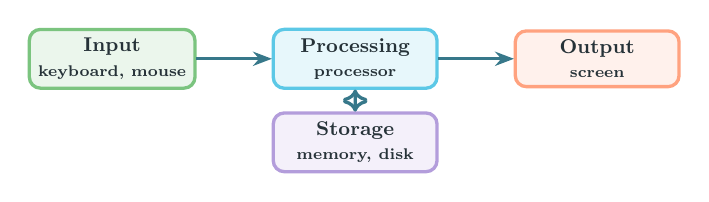
\begin{tikzpicture}[node distance=1.2cm, scale=0.8, transform shape]
        \node[unit=brandGreen, minimum width=2.6cm] (in) {Input\\{\scriptsize keyboard, mouse}};
        \node[unit, minimum width=2.6cm, right=of in] (cpu) {Processing\\{\scriptsize processor}};
        \node[unit=brandOrange, minimum width=2.6cm, right=of cpu] (out) {Output\\{\scriptsize screen}};
        \node[unit=brandPurple, minimum width=2.6cm, below=0.35cm of cpu] (mem) {Storage\\{\scriptsize memory, disk}};
        \draw[sahmT] (in) -- (cpu); \draw[sahmT] (cpu) -- (out); \draw[sahmT, <->] (cpu) -- (mem);
    \end{tikzpicture}
    \end{center}
    \begin{pbox}{\faSmile\quad Analogy}
        A kitchen: data = ingredients, program = recipe, processor = cook.
    \end{pbox}
\end{frame}

\begin{frame}{Example: computing $25 \times 4$}
    \begin{enumerate}
        \item \textbf{Input}: you type 25, $\times$, 4: each key becomes a number code.
        \item \textbf{Storage}: the two numbers are kept in memory.
        \item \textbf{Processing}: the processor runs the multiply instruction: 100.
        \item \textbf{Output}: the result goes to the screen.
    \end{enumerate}
\end{frame}

\begin{frame}{The layers of a computer}
    \begin{center}
    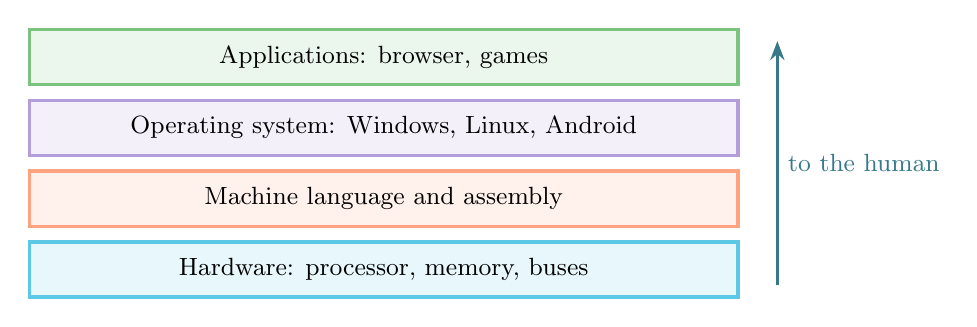
\begin{tikzpicture}
        \node[layer=brandGreen] at (0,1.8) {Applications: browser, games};
        \node[layer=brandPurple] at (0,0.9) {Operating system: Windows, Linux, Android};
        \node[layer=brandOrange] at (0,0) {Machine language and assembly};
        \node[layer=brandTeal] at (0,-0.9) {Hardware: processor, memory, buses};
        \draw[sahmT] (5,-1.1) -- (5,2) node[midway, right, font=\small] {to the human};
    \end{tikzpicture}
    \end{center}
    This course works on the \textbf{two lowest layers}: hardware and assembly.
\end{frame}

\begin{frame}{How does a program run?}
    \begin{enumerate}
        \item The program is a file on the \textbf{disk} (SSD or HDD).
        \item The system \textbf{copies it into RAM}: the disk is too slow for the processor.
        \item The processor reads the instructions \textbf{one after the other} and runs them.
    \end{enumerate}
\end{frame}

\begin{frame}{A short history}
    \begin{center}
    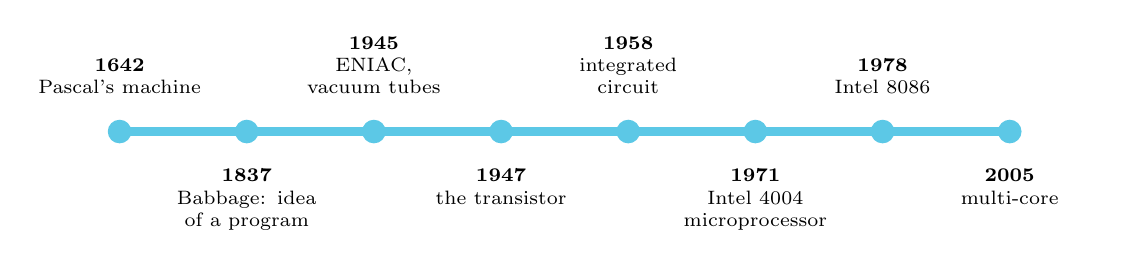
\begin{tikzpicture}[yr/.style={circle, fill=brandTeal, minimum size=0.3cm, inner sep=0pt},
        txt/.style={text width=2.1cm, align=center, font=\scriptsize}, scale=0.95]
        \draw[brandTeal, line width=3pt] (0,0) -- (11.9,0);
        \foreach \x/\y/\t/\p in {0/1642/{Pascal's machine}/above, 1.7/1837/{Babbage: idea of a program}/below,
            3.4/1945/{ENIAC, vacuum tubes}/above, 5.1/1947/{the transistor}/below, 6.8/1958/{integrated circuit}/above,
            8.5/1971/{Intel 4004 microprocessor}/below, 10.2/1978/{Intel 8086}/above, 11.9/2005/{multi-core}/below} {
            \node[yr] (n) at (\x, 0) {};
            \node[txt, \p=0.2cm of n] {\textbf{\y}\\ \t};
        }
    \end{tikzpicture}
    \end{center}
    \begin{tbox}{\faLightbulb\quad Moore's law (1965)}
        The number of transistors on a chip \textbf{doubles about every two years}.
    \end{tbox}
\end{frame}

\begin{frame}{The four generations}
    \begin{center}
    \begin{tabular}{|c|c|c|c|}
        \hline
        \ras{Generation} & \ras{Period} & \ras{Technology} & \ras{Example} \\ \hline
        1st & 1945--1955 & vacuum tubes & ENIAC (30 tons) \\ \hline
        2nd & 1955--1965 & transistor & IBM 7090 \\ \hline
        3rd & 1965--1980 & integrated circuits & IBM 360 \\ \hline
        4th & 1980--today & microprocessor & PC, phone \\ \hline
    \end{tabular}
    \end{center}
    Each generation made the parts \textbf{smaller}, \textbf{faster} and \textbf{less hungry for energy}.
\end{frame}

\begin{frame}{How does a computer count?}
    \begin{tbox}{\faLightbulb\quad Units}
        \begin{itemize}
            \item \textbf{bit}: 0 or 1 \quad \textbf{byte}: 8 bits \quad \textbf{word}: what the processor handles at once (16 bits in the 8086).
        \end{itemize}
    \end{tbox}
    \begin{center}
    \small
    \begin{tabular}{|c|c|c||c|c|c|}
        \hline
        \ras{Dec} & \ras{Bin} & \ras{Hex} & \ras{Dec} & \ras{Bin} & \ras{Hex} \\ \hline
        5 & 0101 & 5 & 10 & 1010 & A \\ \hline
        9 & 1001 & 9 & 12 & 1100 & C \\ \hline
        & & & 15 & 1111 & F \\ \hline
    \end{tabular}
    \end{center}
\end{frame}

\begin{frame}{Converting numbers}
    \begin{gbox}{\faShoePrints\quad \hex{2F} to binary and decimal}
        $2 = 0010$, $F = 1111$, so $\hex{2F} = \bin{0010\,1111}$ \quad and \quad $2 \times 16 + 15 = 47$.
    \end{gbox}
    \begin{gbox}{\faShoePrints\quad \bin{1011} to decimal}
        Weights 8, 4, 2, 1: \quad $8 + 0 + 2 + 1 = 11$.
    \end{gbox}
    \begin{gbox}{\faShoePrints\quad 13 to binary: divide by 2}
        Remainders 1, 0, 1, 1 \quad read backwards: \bin{1101}.
    \end{gbox}
\end{frame}

\begin{frame}{The three main parts}
    \begin{center}
    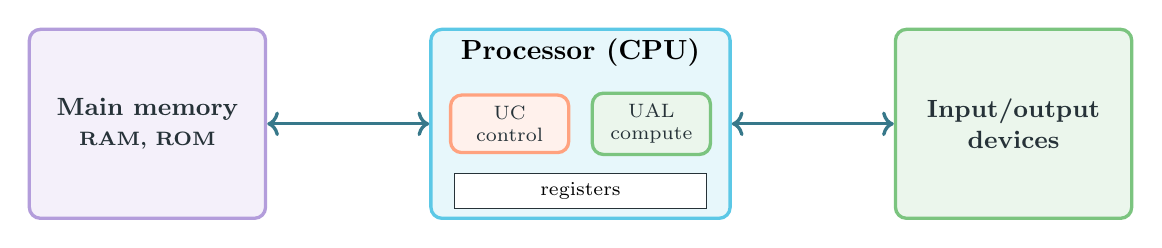
\begin{tikzpicture}
        \node[unit, minimum width=3.8cm, minimum height=2.4cm] (cpu) at (0,0) {};
        \node[font=\bfseries] at (0, 0.9) {Processor (CPU)};
        \node[unit=brandOrange, minimum width=1.5cm, font=\scriptsize] at (-0.9, 0) {UC\\control};
        \node[unit=brandGreen, minimum width=1.5cm, font=\scriptsize] at (0.9, 0) {UAL\\compute};
        \node[draw=brandDark, fill=white, font=\scriptsize, minimum width=3.2cm] at (0,-0.85) {registers};
        \node[unit=brandPurple, minimum width=3cm, minimum height=2.4cm] (mem) at (-5.5,0) {Main memory\\{\scriptsize RAM, ROM}};
        \node[unit=brandGreen, minimum width=3cm, minimum height=2.4cm] (io) at (5.5,0) {Input/output\\devices};
        \draw[sahmT, <->] (cpu) -- (mem); \draw[sahmT, <->] (cpu) -- (io);
    \end{tikzpicture}
    \end{center}
    The \textbf{central unit} = the processor + the main memory.
\end{frame}

\begin{frame}{The Von Neumann model (1945)}
    \begin{center}
    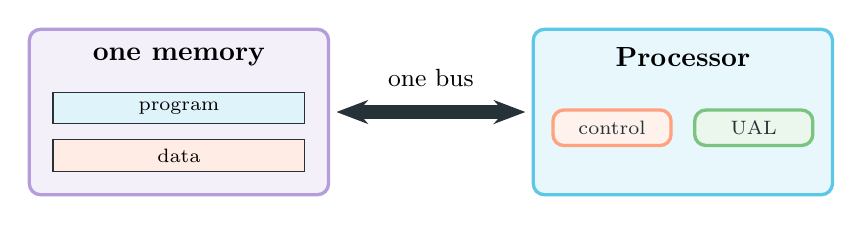
\begin{tikzpicture}
        \node[unit, minimum width=3.8cm, minimum height=2.1cm] (cpu) at (0,0) {};
        \node[font=\bfseries] at (0,0.7) {Processor};
        \node[unit=brandOrange, font=\scriptsize, minimum width=1.5cm] at (-0.9,-0.2) {control};
        \node[unit=brandGreen, font=\scriptsize, minimum width=1.5cm] at (0.9,-0.2) {UAL};
        \node[unit=brandPurple, minimum width=3.8cm, minimum height=2.1cm] (mem) at (-6.4,0) {};
        \node[font=\bfseries] at (-6.4,0.7) {one memory};
        \node[draw=brandDark, fill=brandTeal!20, font=\scriptsize, minimum width=3.2cm] at (-6.4,0.05) {program};
        \node[draw=brandDark, fill=brandOrange!20, font=\scriptsize, minimum width=3.2cm] at (-6.4,-0.55) {data};
        \draw[brandDark, line width=5pt, {Stealth[length=4mm]}-{Stealth[length=4mm]}] (-4.4,0) -- (-2,0);
        \node[font=\small, above] at (-3.2,0.2) {one bus};
    \end{tikzpicture}
    \end{center}
    \begin{itemize}
        \item \textbf{Stored program}: instructions and data in \textbf{the same memory}.
        \item Drawback: one bus, so one transfer at a time: the \textbf{Von Neumann bottleneck}.
    \end{itemize}
\end{frame}

\begin{frame}{The Harvard model}
    \begin{center}
    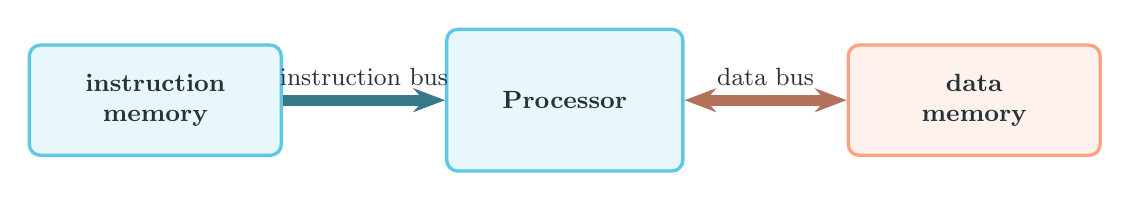
\begin{tikzpicture}
        \node[unit, minimum width=3cm, minimum height=1.8cm] (cpu) at (0,0) {Processor};
        \node[unit=brandTeal, minimum width=3.2cm, minimum height=1.4cm] (im) at (-5.2,0) {instruction\\memory};
        \node[unit=brandOrange, minimum width=3.2cm, minimum height=1.4cm] (dm) at (5.2,0) {data\\memory};
        \draw[tealDeep, line width=4pt, -{Stealth[length=4mm]}] (im) -- (cpu) node[midway, above, font=\small, text=brandDark] {instruction bus};
        \draw[orangeDeep, line width=4pt, {Stealth[length=4mm]}-{Stealth[length=4mm]}] (cpu) -- (dm) node[midway, above, font=\small, text=brandDark] {data bus};
    \end{tikzpicture}
    \end{center}
    \begin{pbox}{\faSmile\quad Analogy}
        A library with \textbf{two doors} instead of one: two queues move at the same time.
    \end{pbox}
\end{frame}

\begin{frame}{Von Neumann or Harvard?}
    \begin{center}
    \begin{tabularx}{0.95\linewidth}{|>{\centering\arraybackslash}p{2.6cm}|C|C|}
        \hline
        \ras{} & \ras{Von Neumann} & \ras{Harvard} \\ \hline
        Memory & one, shared & two, separate \\ \hline
        Speed & slower (bottleneck) & faster \\ \hline
        Cost & simple, cheap & more complex \\ \hline
        Used in & PCs, servers & microcontrollers, DSP \\ \hline
    \end{tabularx}
    \end{center}
    Modern PCs mix both: shared RAM, but separate L1 caches for code and data (\textbf{modified Harvard}).
\end{frame}

\begin{frame}{The processor and its clock}
    \begin{center}
    \begin{tabular}{|c|l|l|}
        \hline
        \ras{Part} & \ras{Job} & \ras{Analogy} \\ \hline
        control unit (UC) & reads and orders & orchestra conductor \\ \hline
        UAL & computes & calculator \\ \hline
        registers & tiny fast memory & scrap paper \\ \hline
    \end{tabular}
    \end{center}
    \begin{gbox}{\faShoePrints\quad A 3 GHz clock}
        $T = \frac{1}{3 \times 10^9} \approx 0.33$ ns per cycle: 300 million cycles while you blink.
    \end{gbox}
\end{frame}

\begin{frame}{Memory: boxes with addresses}
    \begin{columns}
        \column{0.38\textwidth}
        \begin{center}
        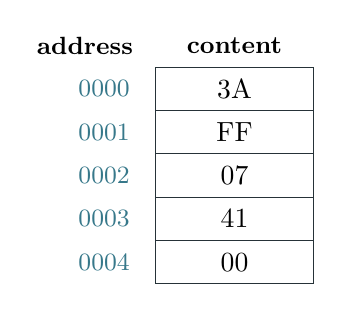
\begin{tikzpicture}[cellx/.style={draw=brandDark, fill=white, minimum width=2cm, minimum height=0.55cm, font=\codefont}]
            \foreach \a/\v [count=\i from 0] in {0000/3A, 0001/FF, 0002/07, 0003/41, 0004/00} {
                \node[cellx] (c\i) at (0, -0.55*\i) {\v};
                \node[font=\codefont\small, text=tealDeep, left=0.2cm of c\i] {\a};
            }
            \node[font=\small\bfseries] at (-1.9, 0.55) {address};
            \node[font=\small\bfseries] at (0, 0.55) {content};
        \end{tikzpicture}
        \end{center}
        \column{0.58\textwidth}
        \begin{itemize}
            \item \textbf{Read}: send an address, get the content.
            \item \textbf{Write}: the new value replaces the old one.
        \end{itemize}
        \begin{pbox}{\faSmile\quad Analogy}
            Address = house number, content = who lives there.
        \end{pbox}
    \end{columns}
\end{frame}

\begin{frame}{Types of memory}
    \begin{center}
    \small
    \begin{tabularx}{0.95\linewidth}{|c|L|c|L|}
        \hline
        \ras{Type} & \ras{Description} & \ras{Power off} & \ras{Used for} \\ \hline
        SRAM & transistors, very fast & erased & cache \\ \hline
        DRAM & capacitors, refreshed & erased & main memory \\ \hline
        ROM & written in the factory & kept & old boot programs \\ \hline
        EEPROM / Flash & erased electrically & kept & BIOS/UEFI, SSD, USB \\ \hline
    \end{tabularx}
    \end{center}
    \textbf{Volatile} memory loses its content without power (RAM); \textbf{non-volatile} memory keeps it.
\end{frame}

\begin{frame}{Computing a memory size}
    \begin{tbox}{\faLightbulb\quad Rule}
        $n$ address lines $\Rightarrow 2^n$ addresses. \quad Size $= 2^n \times$ (size of one box).
    \end{tbox}
    \begin{gbox}{\faShoePrints\quad The 8086: 20 address lines}
        $2^{20} = 1024 \times 1024 = 1\,048\,576$ bytes $= 1$ MB.
    \end{gbox}
    \begin{gbox}{\faShoePrints\quad How many lines for 64 KB?}
        $64 \times 1024 = 2^6 \times 2^{10} = 2^{16}$, so 16 lines.
    \end{gbox}
\end{frame}

\begin{frame}{The three buses}
    \begin{center}
    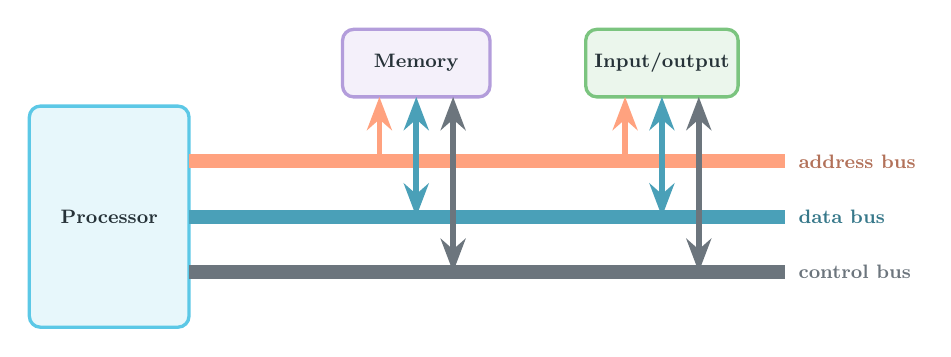
\begin{tikzpicture}[scale=0.78, transform shape]
        \node[unit, minimum width=2.6cm, minimum height=3.6cm] (cpu) at (-5,0) {Processor};
        \node[unit=brandPurple, minimum width=2.4cm, minimum height=1.1cm] (mem) at (0,2.5) {Memory};
        \node[unit=brandGreen, minimum width=2.4cm, minimum height=1.1cm] (io) at (4,2.5) {Input/output};
        \draw[brandOrange, line width=5pt] (-3.7,0.9) -- (6,0.9);
        \draw[brandTeal!80!black, line width=5pt] (-3.7,0) -- (6,0);
        \draw[brandMuted, line width=5pt] (-3.7,-0.9) -- (6,-0.9);
        \node[font=\small\bfseries, text=orangeDeep, anchor=west] at (6.1,0.9) {address bus};
        \node[font=\small\bfseries, text=tealDeep, anchor=west] at (6.1,0) {data bus};
        \node[font=\small\bfseries, text=brandMuted, anchor=west] at (6.1,-0.9) {control bus};
        \foreach \x in {0, 4} {
            \draw[brandOrange, line width=2pt, -{Stealth}] (\x-0.6,0.9) -- (\x-0.6,1.95);
            \draw[brandTeal!80!black, line width=2pt, {Stealth}-{Stealth}] (\x,0) -- (\x,1.95);
            \draw[brandMuted, line width=2pt, {Stealth}-{Stealth}] (\x+0.6,-0.9) -- (\x+0.6,1.95);
        }
    \end{tikzpicture}
    \end{center}
    Address: one way (from the processor). Data and control: both ways.
\end{frame}

\begin{frame}{Example: the processor reads box 0003}
    \begin{enumerate}
        \item It puts 0003 on the \textbf{address bus}.
        \item It sends \textbf{read} (RD) on the \textbf{control bus}.
        \item The memory puts \hex{41} on the \textbf{data bus}, and the processor keeps it.
    \end{enumerate}
    \begin{pbox}{\faSmile\quad Analogy}
        The post office: the shelf number, the parcel, and the words ``give me''.
    \end{pbox}
\end{frame}

\begin{frame}{Bus width}
    \begin{itemize}
        \item Address bus width $\Rightarrow$ \textbf{maximum memory}.
        \item Data bus width $\Rightarrow$ \textbf{bytes moved at once}: 1000 bytes take 1000, 500 or 125 transfers on 8, 16 or 64 bits.
    \end{itemize}
    \begin{center}
    \begin{tabular}{|c|c|c|c|}
        \hline
        \ras{Processor} & \ras{Data bus} & \ras{Address bus} & \ras{Max memory} \\ \hline
        8086 & 16 & 20 & 1 MB \\ \hline
        80386 & 32 & 32 & 4 GB \\ \hline
        x86-64 & 64 & 48 & 256 TB \\ \hline
    \end{tabular}
    \end{center}
\end{frame}

\begin{frame}{Practice}
    \begin{obox}{\faEdit\quad Try it}
        \begin{enumerate}
            \item Convert \hex{3C} to decimal. \hfill \textcolor{brandMuted}{60}
            \item Max memory with a 24-bit address bus? \hfill \textcolor{brandMuted}{16 MB}
            \item Instructions per second at 2 GHz with 4 cycles each? \hfill \textcolor{brandMuted}{500 million}
        \end{enumerate}
    \end{obox}
\end{frame}

\begin{frame}{Summary}
    \begin{tbox}{\faCheckCircle\quad Remember}
        \begin{itemize}
            \item A computer = processor + memory + input/output, linked by buses.
            \item Von Neumann: one memory; Harvard: two memories.
            \item $n$ address lines give $2^n$ addresses.
        \end{itemize}
    \end{tbox}
\end{frame}

\end{document}
